\begin{columns}

\column{0.35\textwidth}
\centering
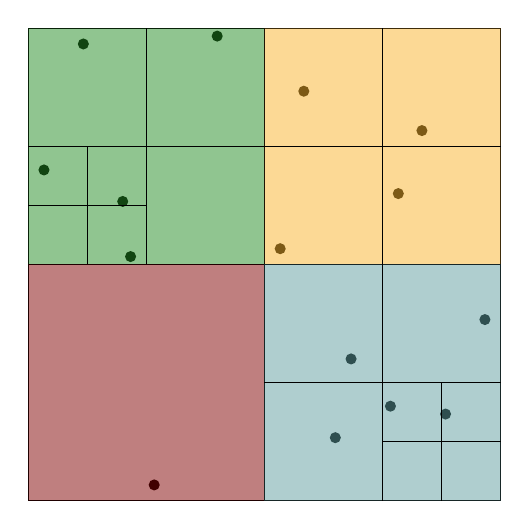
\begin{tikzpicture}
    \onslide<1->{
        \foreach \point in {(2.3,-1.9), (0.5,2.2), (-2.8,1.2),
                            (1.1,-1.2), (-2.3,2.8), (0.2,0.2),
                            (-1.8,0.8), (0.9,-2.2), (2.0,1.7),
                            (1.6,-1.8), (-1.4,-2.8), (1.7,0.9),
                            (-0.6,2.9), (-1.7,0.1), (2.8,-0.7)
        } {\fill \point circle (2pt);}
    }
    \onslide<2->{
        \draw (-3,-3) rectangle (3,3);
    }
    \onslide<3->{
        \draw (-3,0) -- (3,0);
        \draw (0,-3) -- (0,3);
    }
    \onslide<3>{
        \draw[fill=Dandelion,opacity=0.5] (0,0) rectangle (3,3);
        \draw[fill=ForestGreen,opacity=0.5] (-3,0) rectangle (0,3);
        \draw[fill=Maroon,opacity=0.5] (-3,-3) rectangle (0,0);
        \draw[fill=CadetBlue,opacity=0.5] (0,-3) rectangle (3,0);
    }
    \onslide<5->{
        \draw (-3,1.5) -- (3,1.5);
        \draw (-1.5,3) -- (-1.5,0);
        \draw (1.5,3) -- (1.5,-3);
        \draw (0,-1.5) -- (3,-1.5);
    }
    \onslide<6->{
        \draw (-3,0.75) -- (-1.5,0.75);
        \draw (-2.25,1.5) -- (-2.25,0);
        \draw (1.5,-2.25) -- (3,-2.25);
        \draw (2.25,-1.5) -- (2.25,-3);
    }
\end{tikzpicture}

\column{0.65\textwidth}
\centering
\tikzstyle{vertex}=[circle,fill=black!25,inner sep=0pt]
\tikzstyle{vertex1}=[vertex,minimum size=20pt]
\tikzstyle{vertex2}=[vertex,minimum size=12pt]
\tikzstyle{vertex3}=[vertex,minimum size=6pt]
\tikzstyle{vertex4}=[vertex,minimum size=4pt]
\tikzstyle{edge} = [draw,thick,-]
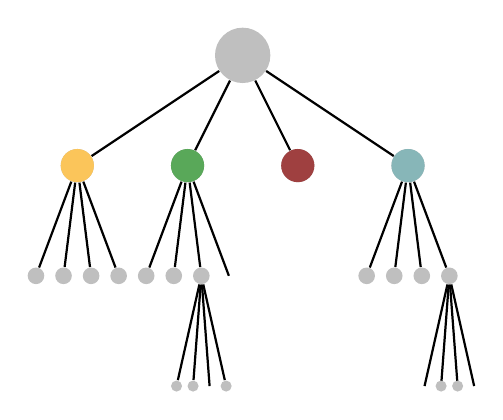
\begin{tikzpicture}[scale=0.7]
    \onslide<2->{
        \node[vertex1] (0) at (0,0) {};
    }

    \onslide<3->{
        \foreach \pos/\name in {(-3,-2)/1, (-1,-2)/2, (1,-2)/3, (3,-2)/4} {
            \node[vertex2] (\name) at \pos {};
            \path[edge] (\name) -- (0);
        }
    }

    \onslide<3>{
        \foreach \pos/\name/\color in {(-3,-2)/1/Dandelion, (-1,-2)/2/ForestGreen, (1,-2)/3/Maroon, (3,-2)/4/CadetBlue}
            \node[vertex2,fill=\color!75] (\name) at \pos {};
    }

    \onslide<5->{
        \foreach \pos/\name in {(-3.75,-4)/11, (-3.25,-4)/12, (-2.75,-4)/13, (-2.25,-4)/14} {
            \node[vertex3] (\name) at \pos {};
            \path[edge] (\name) -- (1);
        }
        \foreach \pos/\name in {(-1.75,-4)/21, (-1.25,-4)/22, (-0.75,-4)/23} {
            \node[vertex3] (\name) at \pos {};
            \path[edge] (\name) -- (2);
        }
        \path[edge] (-0.25,-4) -- (2);
        \foreach \pos/\name in {(2.25,-4)/41, (2.75,-4)/42, (3.25,-4)/43, (3.75,-4)/44} {
            \node[vertex3] (\name) at \pos {};
            \path[edge] (\name) -- (4);
        }
    }

    \onslide<6->{
        \foreach \pos/\name in {(-1.2,-6)/231, (-0.9,-6)/232, (-0.3,-6)/234} {
            \node[vertex4] (\name) at \pos {};
            \path[edge] (\name) -- (23);
        }
        \path[edge] (-0.6,-6) -- (23);
        \foreach \pos/\name in {(3.3,-6)/441, (3.6,-6)/442, (3.9,-6)/443, (4.2,-6)/444} {
            \path[edge] \pos -- (44);
        }
        \node[vertex4] (442) at (3.6,-6) {};
        \node[vertex4] (443) at (3.9,-6) {};
    }
\end{tikzpicture}

\end{columns}